\documentclass{article}
\usepackage[a4paper, total={6.5in, 9in}]{geometry}
\usepackage{amsmath}
\usepackage{graphicx}

\title{Computational Methods: Problem Set 4}
\author{Ian O'Donnell}
\date{\vspace{-5ex}}
\begin{document}
\maketitle

These programs don't converge. Will keep at it. 

\subsection*{Problem One A}

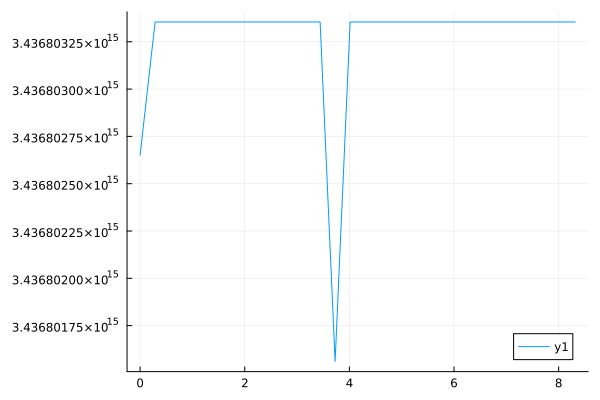
\includegraphics[scale = 0.5]{value.png} \\
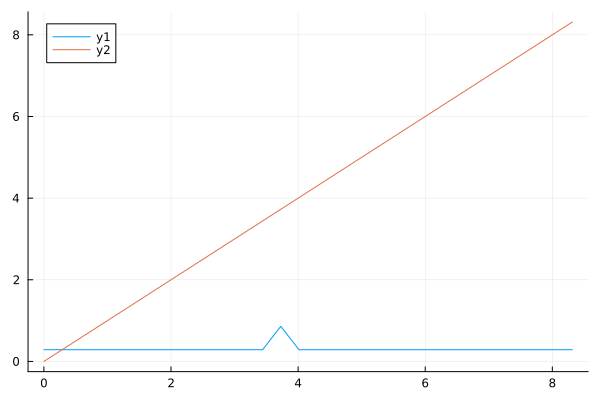
\includegraphics[scale = 0.5]{capital.png}\\
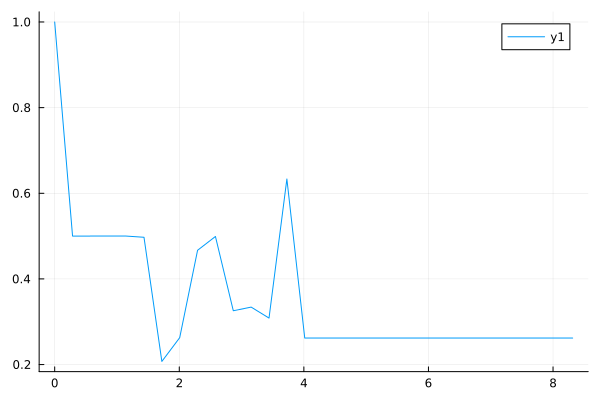
\includegraphics[scale = 0.5]{labour.png}\\
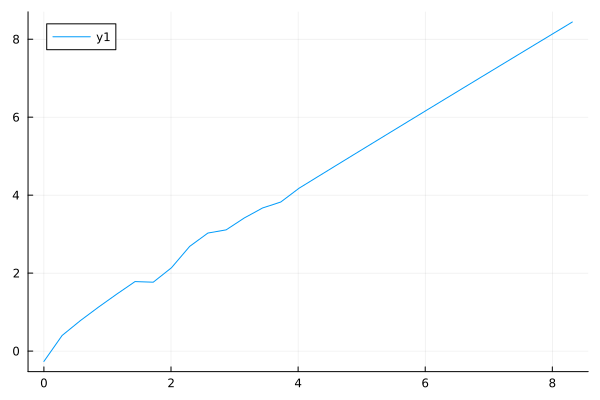
\includegraphics[scale = 0.5]{consumption.png}\\
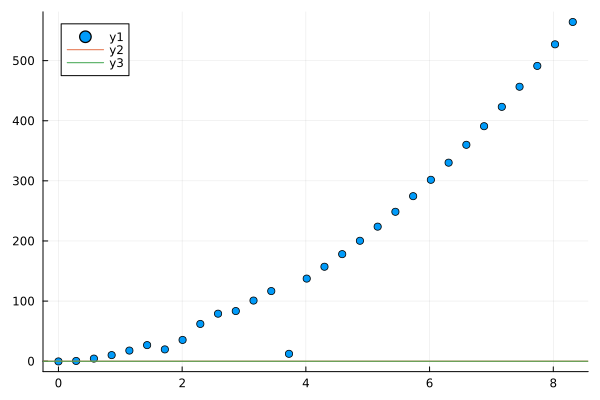
\includegraphics[scale = 0.5]{resid.png}\\

\subsection*{Problem One B}

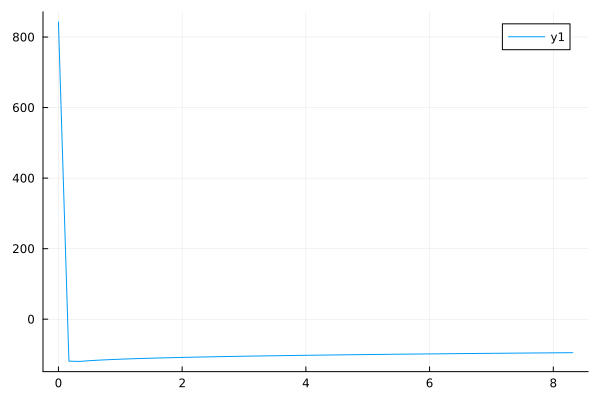
\includegraphics[scale = 0.5]{valueb.png}\\
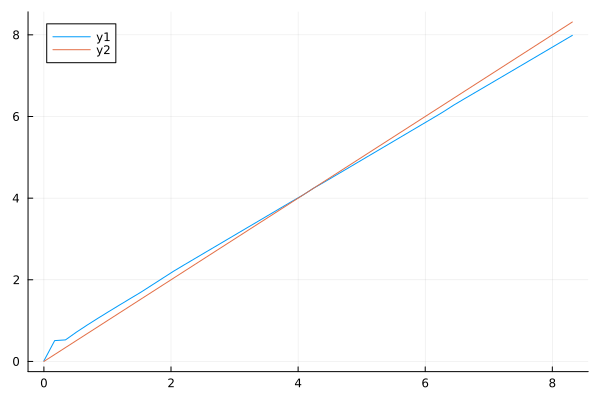
\includegraphics[scale = 0.5]{capitalb.png}\\

\subsection*{Problem One C}

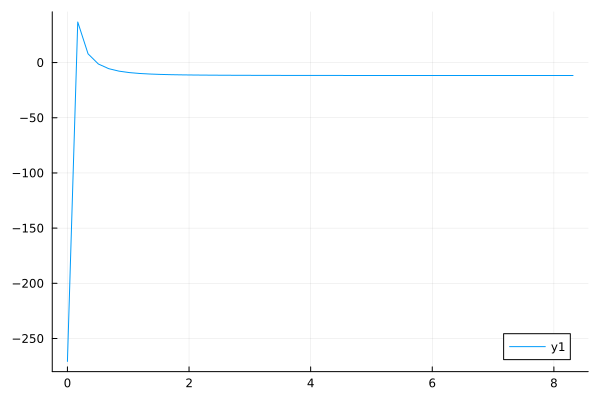
\includegraphics[scale = 0.5]{valuec.png}\\
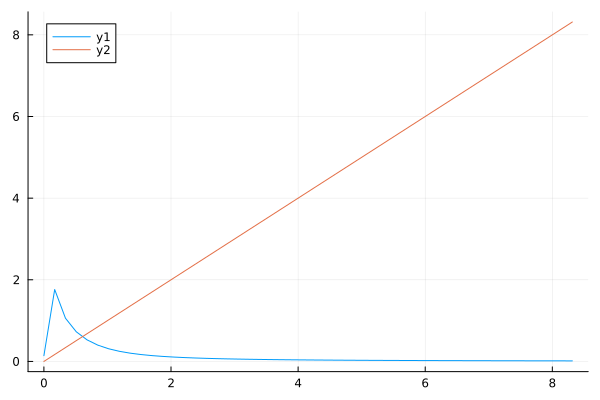
\includegraphics[scale = 0.5]{capitalc.png}\\
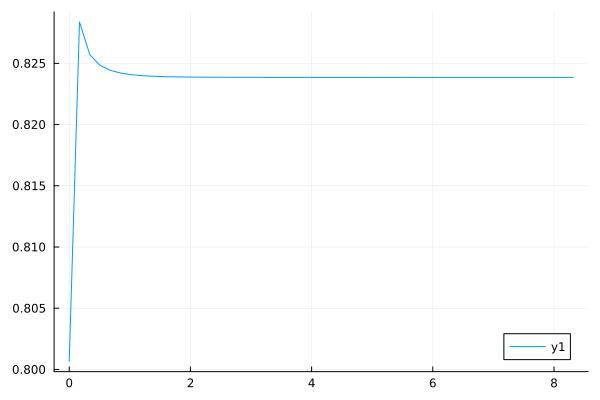
\includegraphics[scale = 0.5]{labourc.png}\\
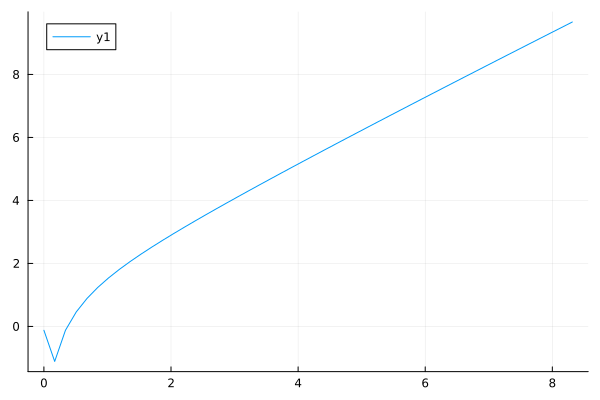
\includegraphics[scale = 0.5]{consumptionc.png}\\
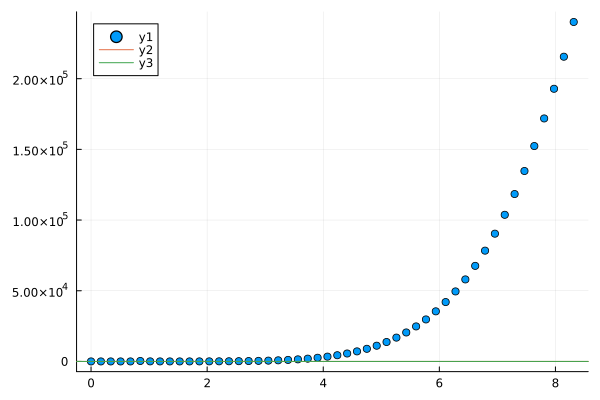
\includegraphics[scale = 0.5]{residc.png}\\
\end{document}